\chapter{Metallurgie}	


\section{Metallurgie Titanlegierungen}
\section{Ti-6242}

	\subsubsection{Zusammensetzung}

					\subsubsection{Zusammensetzung}


Ti-6242 oder Ti-6Al-2Sn-4Zr-2Mo ist eine $\alpha$-$\beta$-Titanlegierung, die  in 1967 von TIMET eingeführt wurde. [Immanuel Freiherr von Thungen]. 
Wie es im Phasendiagramm in Abbildung 1 zu erkennen ist, hat die Legierung Ti6242 bei Raumtemperatur ein hohes Alphaanteil und wird auch deshalb oft als eine Near-$\alpha$-Titanlegierung bezeichnet.

Neben Titan werden bei Ti6242 andere Legierungselemente zulegiert, um bestimmte Eigenschaften zu erreichen. Woraus die Ti-6242 besteht, ist in der Tabelle 1 abzulesen.


\begin{figure}[H]
	\centering
	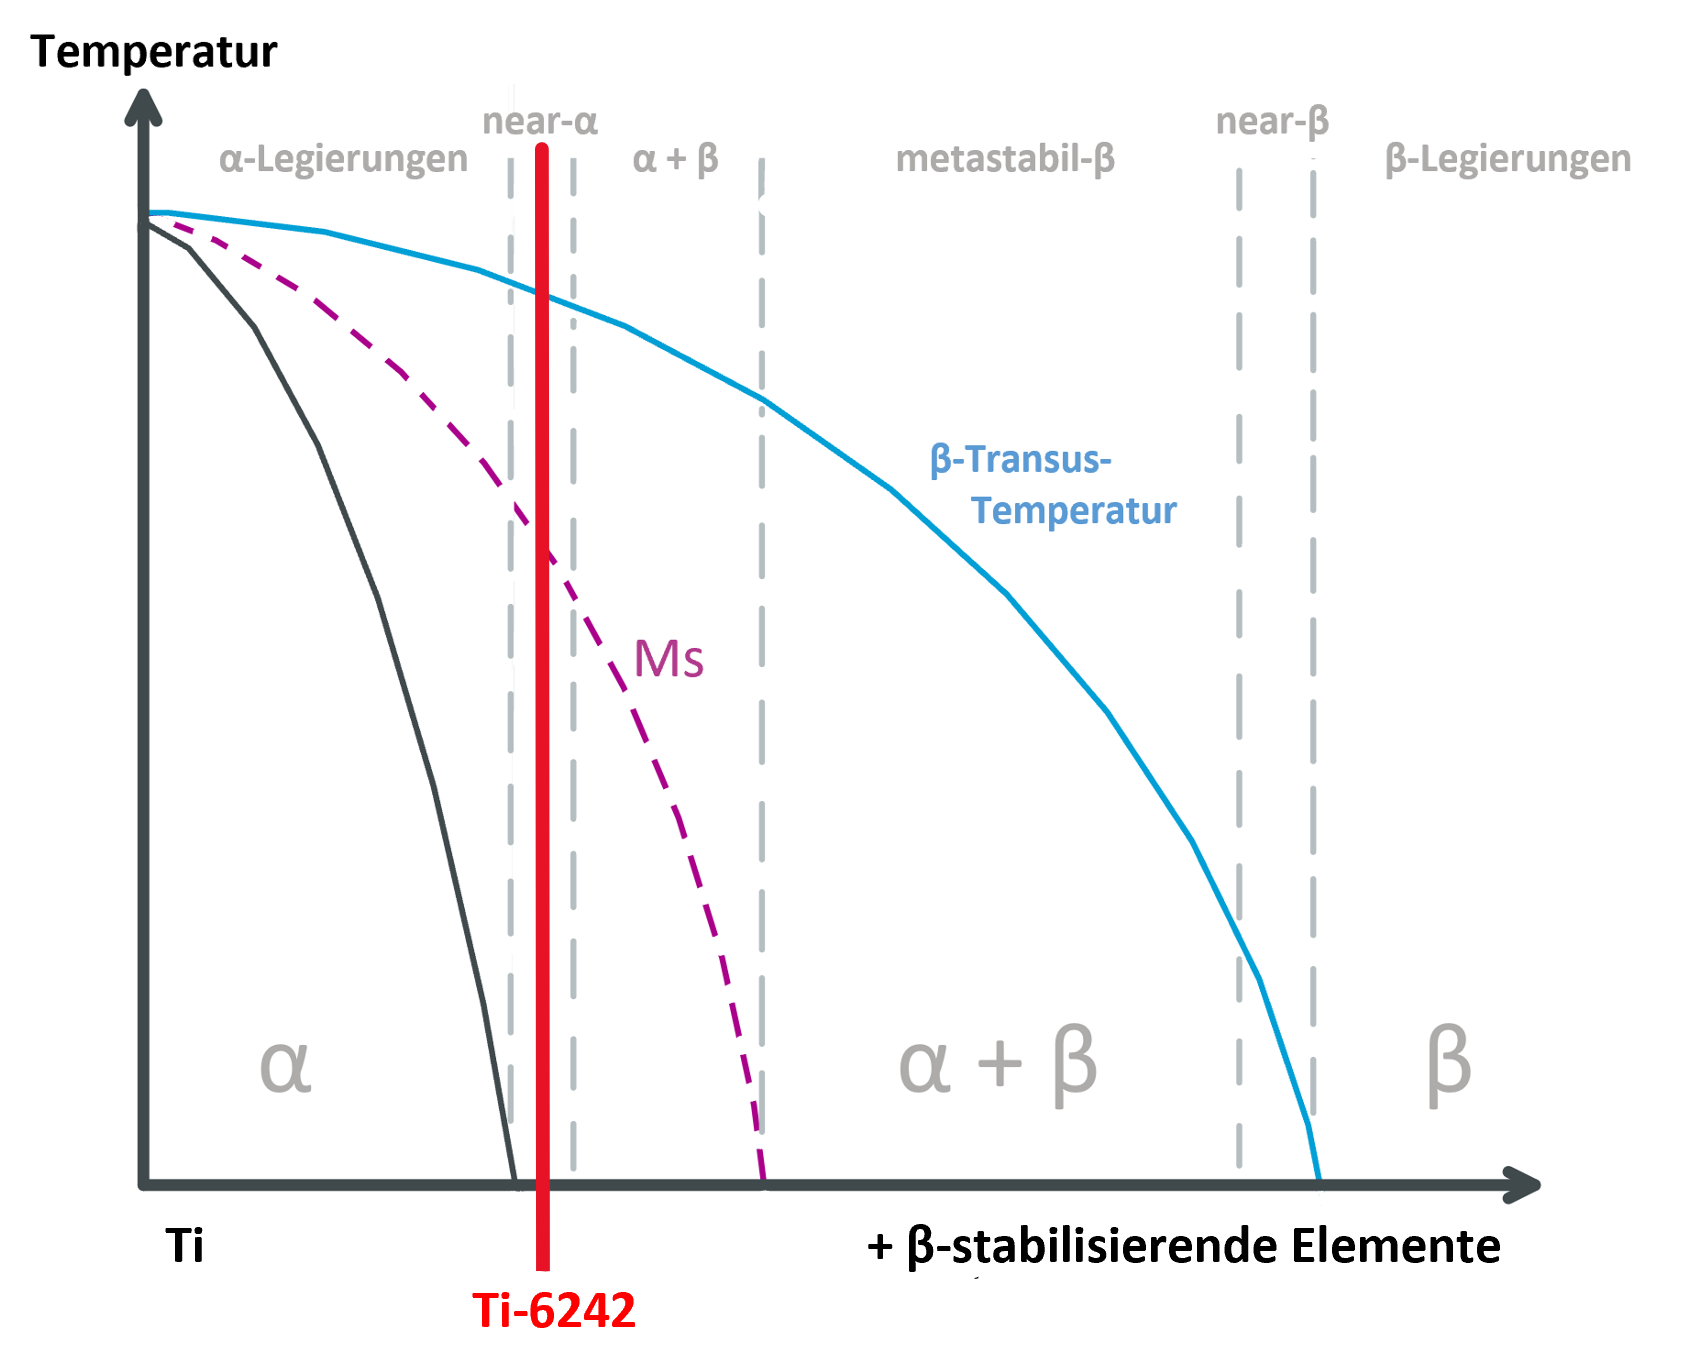
\includegraphics[width=0.5\textwidth]{Bilder/Phasendiagram}
	\caption{Phasendiagramm [Titanium Technical guide]}
	\label{PD-Ti6242}
\end{figure}





\begin{table}[H]
	
	\centering	
	\begin{tabular}{|l |c |c|}
		\hline
		\centering
		\hspace{20ex}Elements \hspace{20ex} & Min \%Gwt. & Max \%Gwt.\\
		\hline
		Aluminium&5,5&6,5\\
		Tin&1.80&2.20\\
		Zirconium&3.60&4.40\\
		Molybdenum&1.80&2.20\\
		Silicon &0.06&0.13\\
		Iron&-&0.25\\
		Oxygen&-&0.15\\
		Carbon&	-&	0.05\\
		Nitrogen&-&0.03\\
		Hydrogen&-&0.0125\\
		
		Titanium &&Remainder\\
		\hline
	\end{tabular}
	\caption{Zusammensetzung von Ti-6242 [Titanium : Technical guide]}
\end{table}


Die Ti6242S ist eine Optimierung von Ti6242, die erst in den 1970er Jahren  entwickelt wurde. Dieser wurde zusätzlich Silizium in kleinen Mengen zulegiert, um die Resistenz gegen Kriechen vor allem bei hohen Temperaturen durch die Bildung von Siliziden ($Ti_5Si_3$) zu erhöhen.  [Titanium and Titanium Alloys : Fundamentals and apps]. 

Verzeichnis : [Immanuel Freiherr von Thungen] - Immanuel Freiherr von Thungen. Effet dwell: relation microstructure-microtexture-propriétés mécaniquesdel’alliagedetitaneTi6242. Autre. ISAE-ENSMAEcoleNationaleSupérieuredeMécanique et d’Aérotechique - Poitiers, 2016. Français. NNT: 2016ESMA0027 .  tel-01486574
[Titanium and Titanium Alloys : Fundamentals and apps] Williams J. C., Belov A. F., eds.: Titanium and Titanium Alloys, Plenum Press, New York, USA, (1982) 


\subsubsection{Kristallstruktur}

Ti6242 wird klassischerweise in der bimodalen oder Duplex-Struktur eingesetzt die nach einer typischen Wärmebehandlung , erklärt in Abbildung \ref{WB} , erreicht  werden kann.

\begin{figure}[H]
	
	\centering
	
	{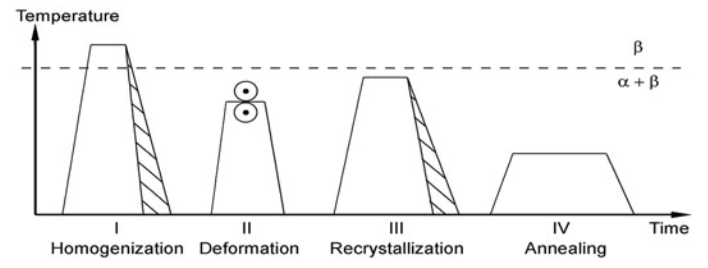
\includegraphics[width=1\textwidth]{Bilder/WB}}			
	\caption{Schematic processing route for bi-modal microstructures alpha+$\beta$-titanium alloys )}
	\label{WB}
\end{figure}
Nach dem Deformationsvorgang wandelt sich bei der Erwärmung von Raumtemperatur  auf \hspace{1ex} T1<$T_{\beta}$  ein Anteil von der $\alpha$-Phase in $\beta$ um. Nach 1-2h werden die Werkstücke wieder auf Raumtemperatur luftgekühlt.
Dabei wandelt sich das $\beta$ unter Einfluss der Diffusion in $\beta$ + $\alpha$-Lamellen um.

\begin{figure}[H]
	\centering
	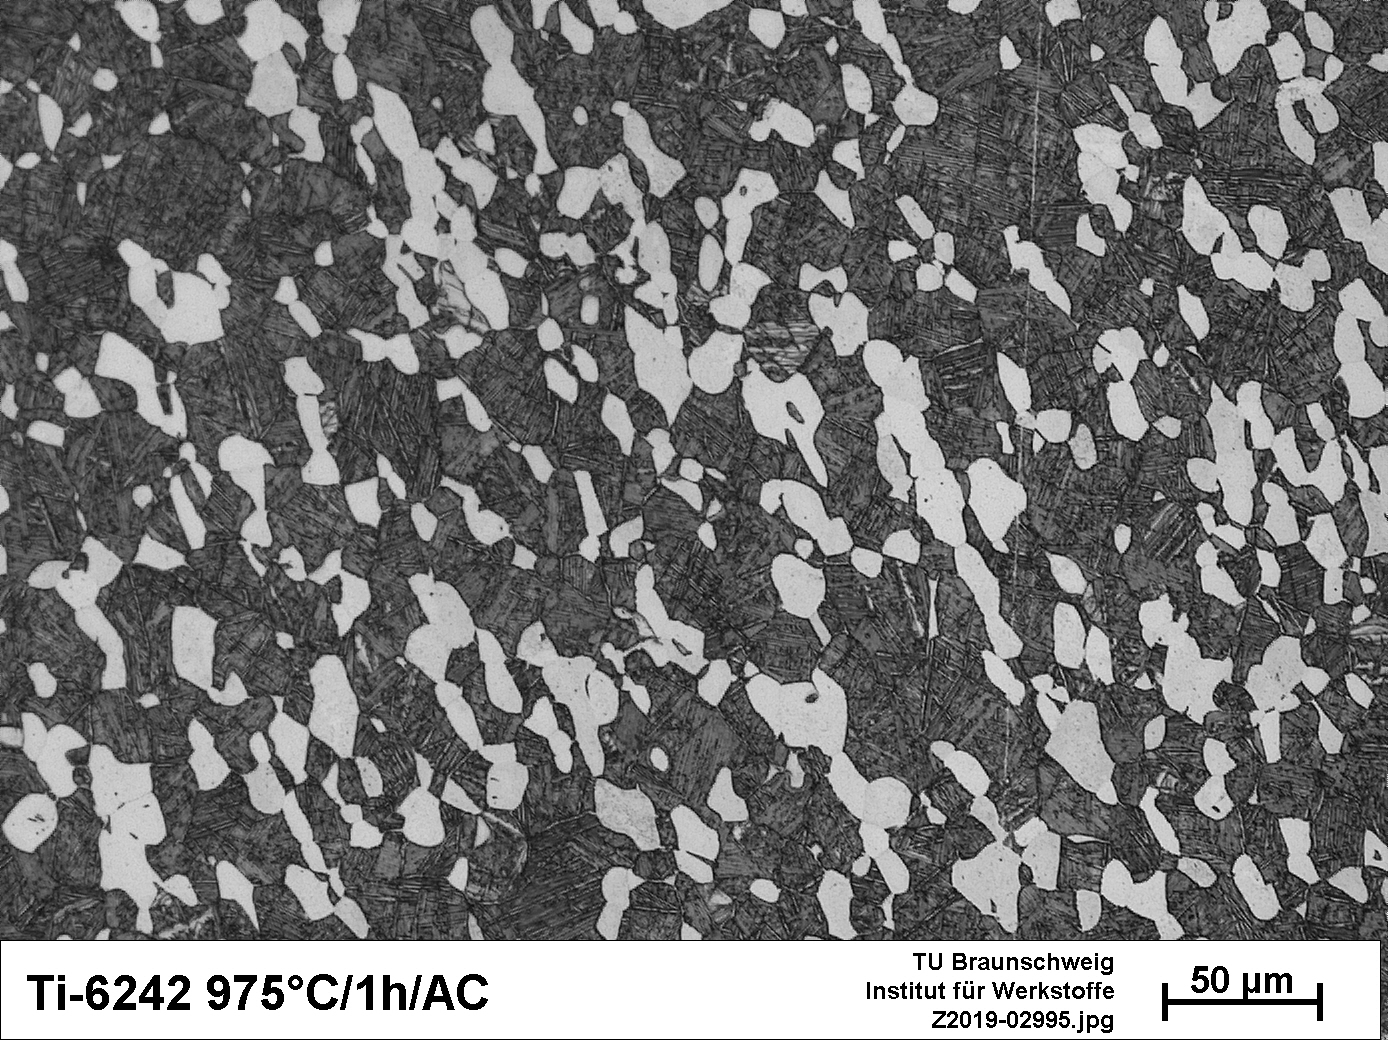
\includegraphics[width=0.9\textwidth]{Bilder/LM-975-1h-AC}
	\caption{}
	\label{L.M}
\end{figure}


Als letzte Wärmebehandlung wird klassischerweise  Ti6242 oder Ti6242S für  8 h bei 595°C angelassen. Dieser Schritt sorgt dafür, dass sich $\alpha_2$ ($Ti_3Al$) in der $\alpha$-Phase ausscheidet und die dadurch weiter verstärkt. Der Temperaturbereich hängt dabei von der Solvus-Temperatur von $\alpha_2$ in $\alpha$, die ca. 650°C beträgt.(Titanium lütjering )
Für besonders gute Kriechverhalten bei hohen Temperaturen, wird auch die Solvus-Temperatur von Si berücksichtigt, die knapp unter 600°C liegt. Silizide ($Ti_5Si_3$) können sich aufgrund ihrer komplexen Kristallstruktur dann in den Korngrenzen ausscheiden und Kornbewegungen verhindern.


\begin{figure}[H]
	\centering
	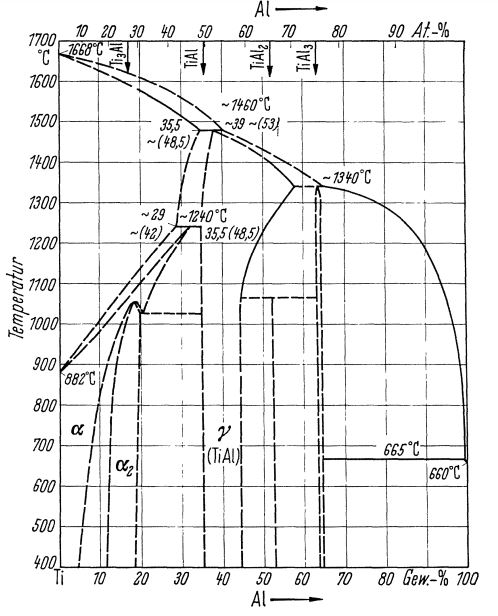
\includegraphics[width=0.6\textwidth]{Bilder/TiAl}
	\caption{Phasendiagramm von Ti-Al . [Titan Titanöegierungen, Ulrich Zwicker]}
\end{figure}
+ Phasendiagram Mo-Ti
Wärmebehandlungen von Ti6242 und deren Einflüssen werden in den nächsten Kapiteln noch genauer diskutiert.


\subsubsection{ Physikalische und mechanische Eigenschaften }

Die Tabelle in Abbildung \ref{Phy.eig.} fasst ein paar physikalische Kennwerte vom Ti-6242 zusammen.
\newline
\textit{	Referenzen : 
	Metals Handbook, Vol.2 - Properties and Selection: Nonferrous Alloys and Special-Purpose Materials, ASM International 10th Ed. 1990.				
	Metals Handbook, Vol. 3, Properties and Selection: Stainless Steels, Tool Materials and Special-Purpose Metals, Ninth Edition, ASM Handbook Committee., American Society for Metals, Materials Park, OH, 1980.				
	Structural Alloys Handbook, 1996 edition, John M. (Tim) Holt, Technical Ed; C. Y. Ho, Ed., CINDAS/Purdue University, West Lafayette, IN, 1996. }

\begin{table}[H]
	\centering	
	\begin{tabular}{l c}
		
		Physikalische Eigenschaften & \\
		\hline
		Dichte& 4,54 g/$cm^3$\\
		Wärmeleitfähigkeit & 7 W/m.K \\
		Spezifische Wärmekapazität & 0.460 J/g.K\\
		Schmelzpunkt & 1700°C \\
		$T_{\beta}$ &  995°C $\pm$ 15°C \\
		\hline
		
	\end{tabular}
	\caption{Physikalische Kennwerte von Ti6242 : ???]}
	\label{Phy.eig.}
\end{table}


Die mechanischen Eigenschaften von Titanlegierungen, wie bereits im ersten Kapitel erklärt wurde, hängen auch stark von den verschiedenen Wärmebehandlungen ab, die die Gefügestruktur des Werkstoffes  verändern und so auch sein thermomechanisches Verhalten.
Als eine Near-$\alpha$Titan Legierung, ist Ti6242 zum größten Teil $\alpha$(90-95\%)(Siehe Phasendiagramm in Abbildung \ref{PD-Ti6242}). Da die Diffusionsrate bei $\beta$-Strukturen höher ist als bei $\alpha$Strukturen weist Ti6242 eine bessere Stabilität bei höheren Temperaturen auf. (Aerospace Materials and Material Technologies ) 

\begin{table}[H]
	\centering	
	\begin{tabular}{|c| c| c| c| c| c|}										
		\hline
		$T_{\beta}$ & Härte[HV] & E-Modul [Gpa]& YS [Mpa]&TS[Mpa]& El \% \\
		\hline
		995&340&114&990&1010&13\\
		\hline
	\end{tabular}
	\caption{Physikalische Kennwerte von Ti6242S [Titanium and Titanium alloys  : Fundamentals and apps.]}
	\label{Mec.}
\end{table}

Die $\alpha$-$\beta$-Transformationstemperatur $T_{\beta}$ von Ti-6242 liegt bei 995°C $\pm$ 15°C . Die Abweichung hängt  von den Anteilen der verschiedenen Legierungselementen ab. Wie bereits im ersten Kapitel beschrieben wurde, stabilisieren  Al, O , N und C die $\alpha$Phase und erhöhen im Gegensatz zu Mo  {$T_{\beta}$}.
Aufgrund des niedrigen Mo-Gehalts von Ti6242 liegt ihre Betat-trans-Temperatur oberhalb der von Reinem Titan, die bei 882 $\pm$ 2°C liegt.


\begin{figure}[H]
	\centering
	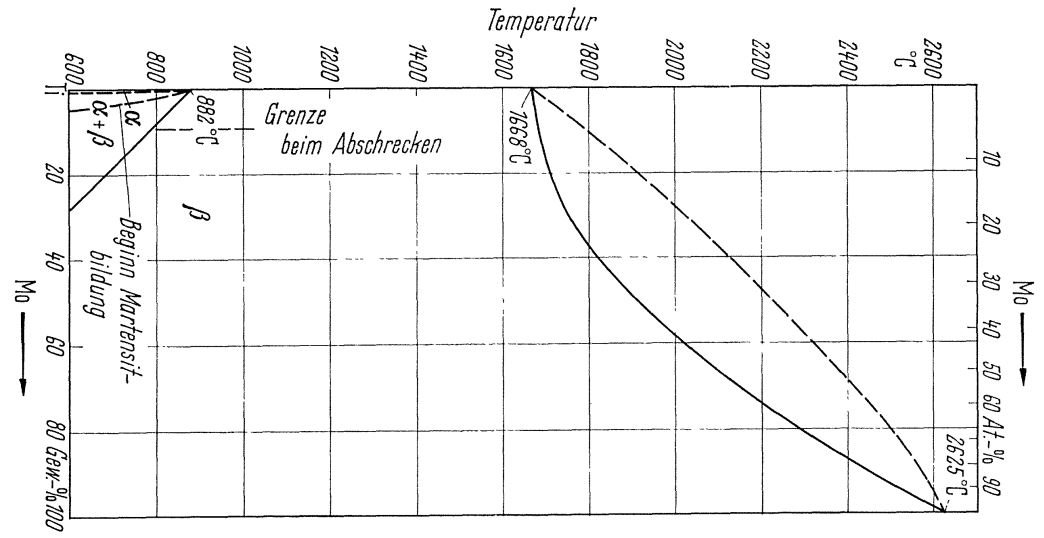
\includegraphics[width= 0.6\textwidth]{Bilder/TiMo}
	\caption{Phasendiagramm Ti-Mo [Titan titanlegierungen Zwickers]}
	\label{TiMo}
\end{figure}

\begin{table}[H]
	\small
	\tabcolsep=0.09cm
	\centering	
	\begin{tabular}{|c |c |c|c |c|}
		\hline
		\centering
		Thickness[mm] & Tensile strength [MPa] & Yield strengh [MPa] & Elongation[\%]& Reduction in Area [\%]. \\
		\hline
		25-50&1000&930&14&33\\
		102&1000&930&12&30\\
		205&1035&940&12&28\\
		330&1000&825&11&21\\
		
		\hline
	\end{tabular}
	\caption{Elatische Eigenschaften bei Raumtemperatur von Ti6242Si (Annealed 1h 954°C/AC + 8h/600°C/AC )  [Titanium : Technical guide]}
	\label{Mecprop}
\end{table}






%	Für den Einsatz in der Luftfahrt sind aber auch spezielle mechanische  Eigenschaften wie zB eine hohe Festigkeit und Duktilität, eine hohe Kriech- und Korrosionsbeständigkeit bei relativ hohe Temperaturen gesucht.   

Alle sekundären Fertigungsverfahren, die für die Herstellung von Bauteilen erforderlich sind   wie zB. Biegen, Fräsen und Schweißen können Eigenschaften von Titan oder Titanlegierungen stark beeinflussen  und müssen daher mitberücksichtigt werden.




\subsubsection{Verwendung}


Die Kombination von der Festigkeit der ($\alpha$+$\beta$)-Gefüge mit der relativ hohen Kriechbeständigkeit der $\alpha$-Strukturen macht von Ti6242/Ti6242S eine \textit{High Temperature Ti-Alloy}.

Wegen dieser Eigenschaften werden Ti6242/Ti6242S hauptsächlich in der Luftfahrt eingesetzt. Vor allem bei rotierenden Teilen im Triebwerk, wo  hohe Kriechbeständigkeit, Ermüdungsresistenz  neben eine hohe metallurgische Stabilität bei hohen Temperaturen erforderlich sind. 
Ti6242-Bauteile können in Temperaturen bis zu 500-550°C eingesetzt werden. [Titanium and itanium alloys : fundamentals and apps]
Ti6242 wird z.B. in der Herstellung von Hochdruckverdichterschaufeln, Turbinenschaufeln und Nachbrennern verwendet, wo neben den oben erwähnten Eigenschaften auch die Korrosionsbeständigkeit bei hohen Temperaturen erforderlich ist. \newline



\begin{figure}[H]
	\centering
	\subfloat[Compressor spoolfor GE CF6 class engine using inertia welding toconnect the individual stages:front (smaller)five stages: Ti–6Al–4V; rear two stages:Ti-6242 ]
	{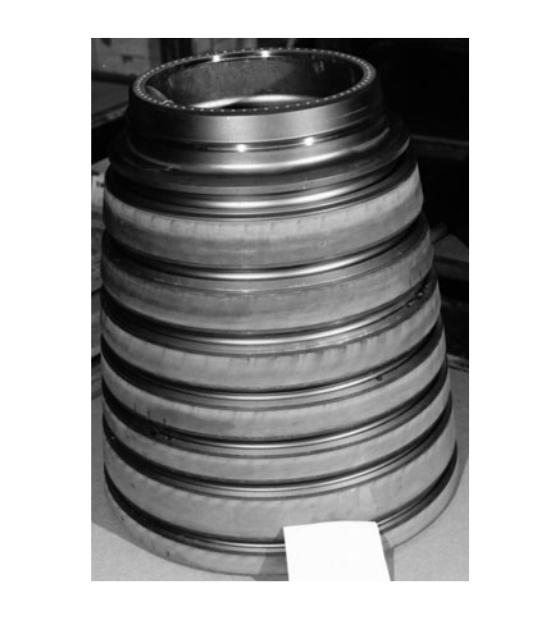
\includegraphics[width=0.45\textwidth]{Bilder/Compressor spool}}
	\hspace{1ex}
	\subfloat[Impeller used in asmall engine for regional jets, diameter 35 cm. The alloy is Ti-6242 with a bi-modalmicrostructure]
	{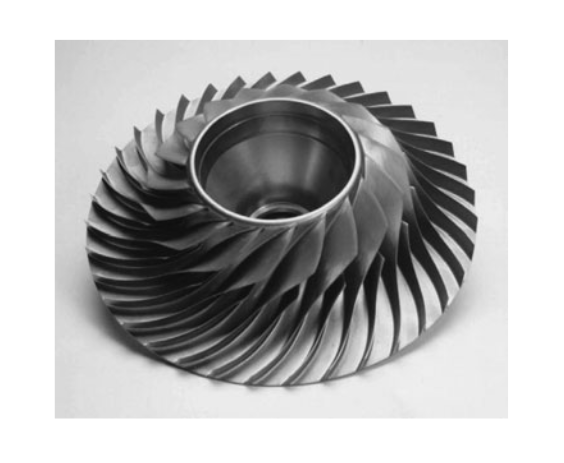
\includegraphics[width=0.45\textwidth]{Bilder/Impeller}}
	
	\subfloat[Bläser und Verdichter des JT9D-Triebwerkes. das zu 28 % des Fluggewichtes aus
	Titan und Titanlegierungen besteht. Bläser aus TiAI6V4. Verdichter mit zunehmender
	Temperatur aus TiAI6V4, TiAl811folVI und TiAl6Zr4Sn2Mo2 [T 19b].]
	{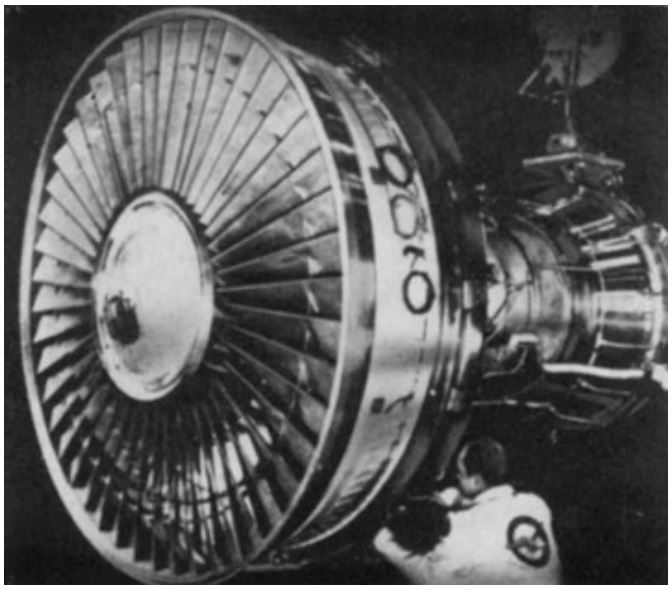
\includegraphics[width=0.45\textwidth]{Bilder/Titan}}
	\caption{Beispiele von Einsatzbereiche von Ti-6242 (Aerospace Materials and Material Technologies )}
\end{figure}




